\subsection{Evaluating Performance Comparison Results}

 \begin{figure}[H]
    \begin{center}
    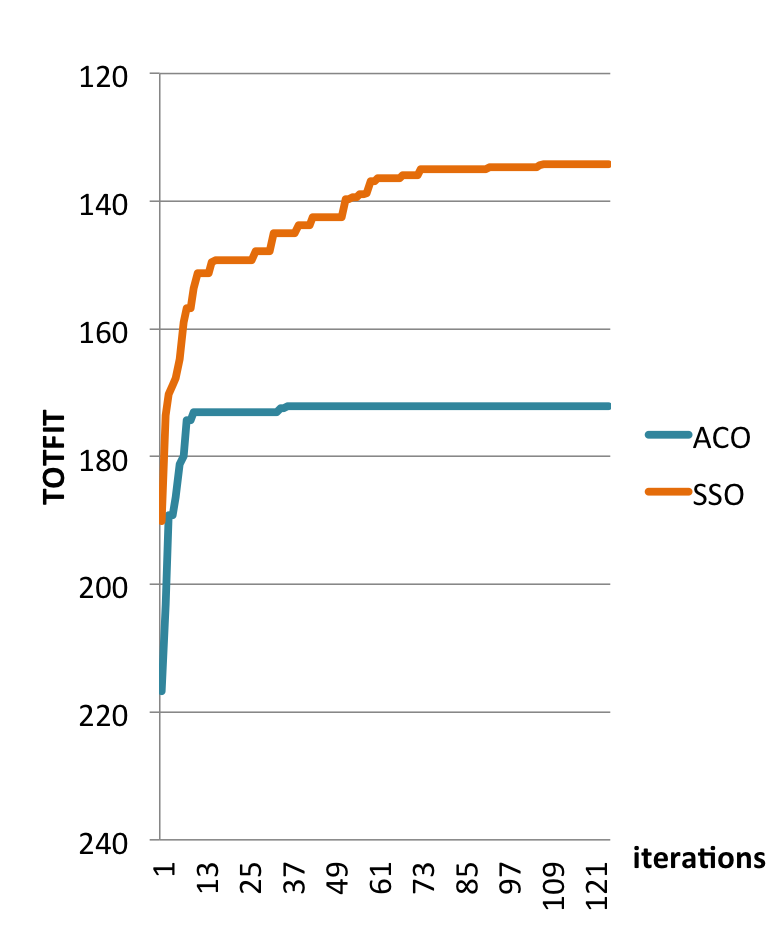
\includegraphics[width=3in]{assets/acovsssoNEW.png}
    \end{center}
    \caption{Evolution of TOTFIT for ACO and SSO }
    \label{fig:acovssso} 
    \end{figure}

Figure \vref{fig:acovssso} shows the average growth in the TOTFIT value for each iteration of ACO and SSO. 10 runs for each algorithm is run. For each iteration, the average $TOTFIT$ value among each run is recorded. 

ACO stuck at local optima. As seen in Figure \vref{fig:acovssso} SSO manage too get out of local optima. Notion of global best solution, crazy ants, following ants reward best edges, memory etc.

 \begin{table}[H]
    \centering
    \begin{tabular}{|l||l|l|l|l|l|}
    \hline
    Route Set & $d_0(\%)$ & $d_1(\%)$ & $d_2(\%)$ & $d_{unsat}(\%)$ & $ATT$ \\
    \hline
    4 & 81.92 & 16.13 & 1.86 & 0.09 & 10.43\\
    \hline
    6 & 87.17 & 12.0 & 0.82 & 0.01 & 10.11\\
    \hline
    7 \\
    \hline
    \end{tabular}
    \caption {Evaluating increase of Route Sets}
    % 50 runs
    \label{table:performanceComparison_ACOSSOBEST}
    \end{table}

\subsection{Evaluating Scalability Results}
\subsection{Evaluating Neo4J}
Limitations

%Metaheuristics, like ACO, requires a good initial parameter setting to solve concrete problems optimally. As mentioned in the 

%\emph{\color{blue} TODO:}
%Punkter vi må huske på:
%\begin{itemize}
%\item The parameter settings will be optimized for the Mandl network with 4 routes?
%\item 0\% crazy ants gave worse results than both 5\% and 10\% CA: some crazy ants is better than none. But, as we see in the results, more than 10\% CA gives worse results than 0\% CA, \emph{\color{blue} it does not mean the more crazy ants, the better results regarding the final results. But some CA is good.}
%\end{itemize}